\chapter{Shared Memory Architectures}
\label{ch:04/shared-memory-architectures}

Shared Memory Architectures are a type of MIMD architecture where all processors share the same memory space, and can access it directly. This is the most common architecture for multi-core processors (\textit{``multiprocessors''}).

They mirror the Von Neumann architecture, with multiple processors sharing the same memory space.

\section{Von Neumann Bottleneck}

\begin{definition}[von Neumann Bottleneck]
   The \textit{von Neumann bottleneck} is a limitation on throughput caused by the standard personal computer architecture. The term is named for John von Neumann, who is credited with developing the von Neumann architecture, in which programs and data are stored in the same memory. \ul{The bottleneck refers to the limited data transfer rate between a computer's CPU and memory compared to the amount of memory.}
\end{definition}

\begin{figure}[htbp]
   \centering
   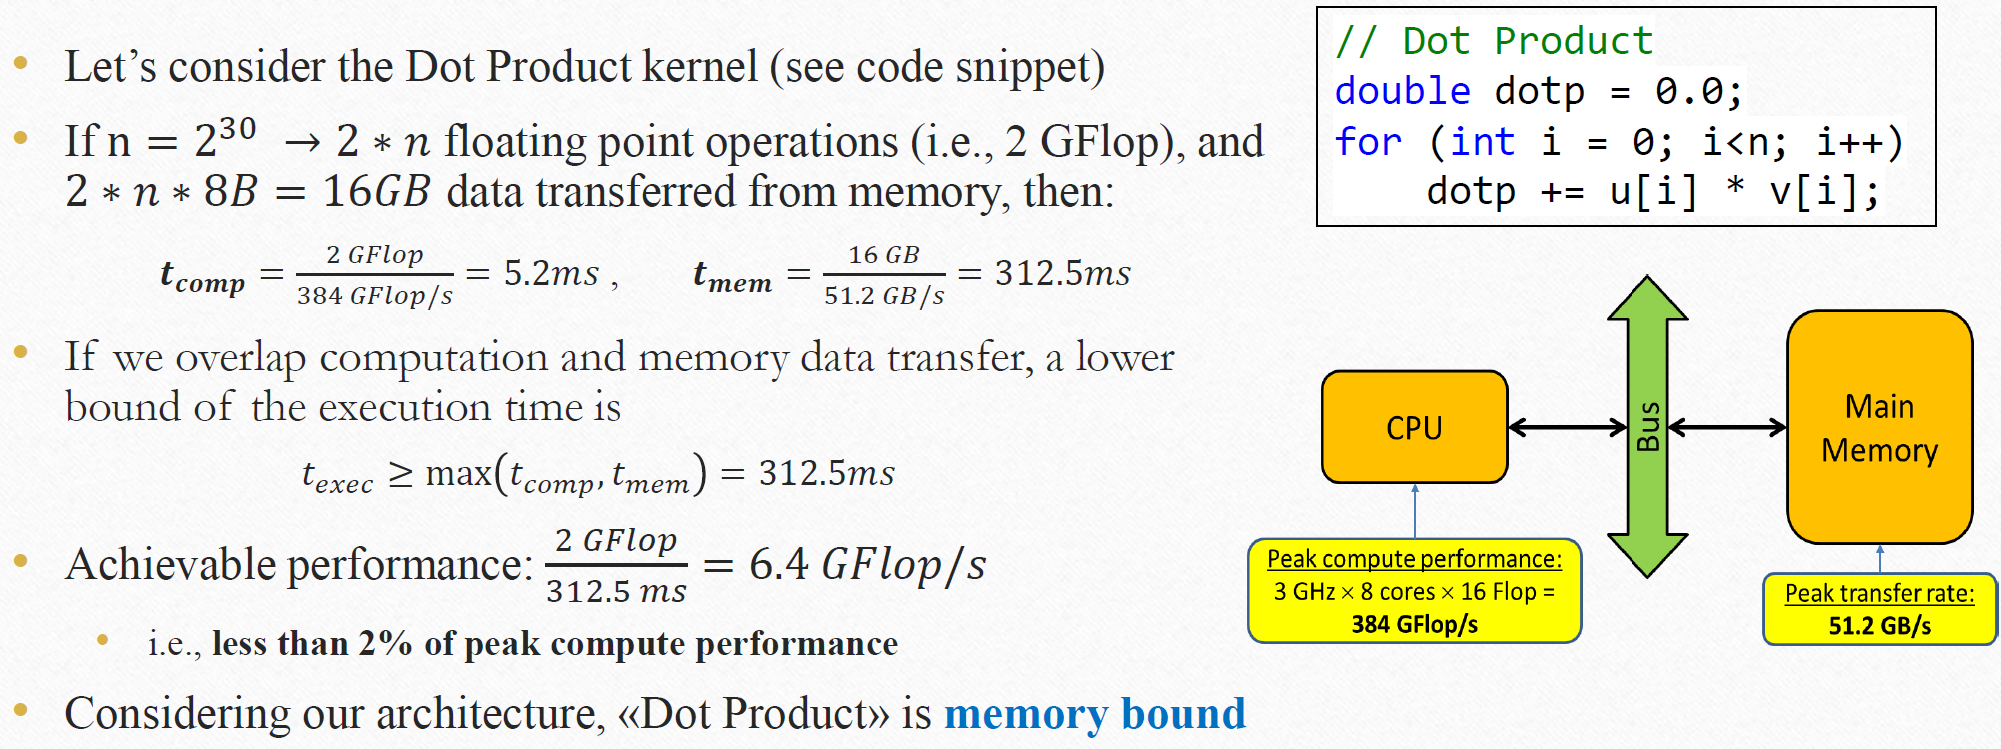
\includegraphics{images/04/neumann_example.png}
   \caption{von Neumann Bottleneck example}
   \label{fig:04/neumann_example}
\end{figure}

In the example in Figure \ref{fig:04/neumann_example}, the CPU is waiting for the data to be loaded from memory, which is a slow operation, leading to \ul{exploiting only the 2\% of the CPU capabilities.}

\subsection{Caches}

\begin{paracol}{2}
   Back in the day, the solution was to \textit{``move the data closer to the CPU''}, introducing \textbf{memory hierarchy} and \textbf{caches}.

   Usally, L1 and L2 are private to each core, while L3 is shared among all cores.
   \switchcolumn
   
   \begin{figure}[htbp]
      \centering
      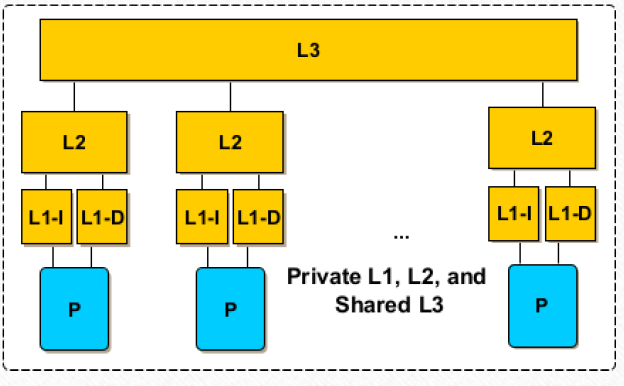
\includegraphics{images/04/caches_hierarchy.png}
      \caption{Caches hierarchy}
      \label{fig:04/caches_hierarchy}
   \end{figure}
\end{paracol}

If a matrix of the previous example in Fig. \ref{fig:04/neumann_example} is entirely stored in cache, then the achievable performance is \ul{223 GFLOPS, which is about 60\% of the peak power.}

If the matrices do not fit in the cache, the performance drops since we need to trap to the main memory to fetch missing data.\\
So, the problem shifts to understand how to exploit the cache to its fullest.

\section{Locality Principle}

The locality principle is the driving force that makes the cache work. Locality increases the probability of reusing data blocks that were previously moved from level $n$ to level $n-1$.
\begin{itemize}
   \item \textbf{Temporal Locality}: if a data is accessed, it is likely to be accessed again soon.
   \note{Cache mapping strategy (Direct/associative) and the replacement policy (LRU, FIFO, Random etc.) are crucial to exploit temporal locality.}
   \item \textbf{Spatial Locality}: if a data is accessed, it is likely that nearby data will be accessed soon.
\end{itemize}

\subsection{Measuring CPU time with caches}
\begin{equation}
   CPU_{time} = ClockCycles \cdot ClockCycleTime = IC \cdot ClockCycleTime
\end{equation}
\begin{itemize}
   \item IC: Instruction Count (number of instructions executed)
   \begin{itemize}
      \item $IC = IC_{CPU} + IC_{MEM}$
   \end{itemize}
   \item CPI: Cycles Per Instruction
   \begin{itemize}
      \item $CPI = \dfrac{ClockCycles}{IC}$
      \item $CPI = \dfrac{IC_{CPU}}{IC} \cdot CPI_{CPU} + \dfrac{IC_{MEM}}{IC} \cdot CPI_{MEM}$ where $CPI_{CPU}$ are the average cycles per ALU instruction and $CPI_{MEM}$ are the average cycles per memory instruction.
      \item Considering that each memory instruction may generate a cache hit or miss with a given probability, and naming $HitRate$ the probability of a cache hit, we can write 
      \begin{equation}
         CPI_{MEM} = HitRate \cdot CPI_{MEM - Hit} + (1-HitRate) \cdot CPI_{MEM - Miss}
      \end{equation}
   \end{itemize}
\end{itemize} 

\subsection{Cache Algorithms}
\begin{enumerate}
   \item \textit{What do we load from main memory?}
   \item \textit{Where do we store it in the cache?}
   \item \textit{Cache is full, what should we evict?}
\end{enumerate}